%% How To get it to compile in TexWorks (CAC, 5/2013)
%% Go to this site: 
%% https://code.google.com/p/texworks/wiki/AdvancedTypesettingTools#latex_->_dvips_->_ps2pdf
%% and follow the directions.
% Here is some of the text from this page:
%Configuring LaTeX for .ps output is not straight-forward. TeXworks only supports running a single command at once, 
%but for producing .ps files one needs to call both "latex" and "dvips". 
%To be able to do that, you need to create a simple script, the content of which is platform dependent (see below). 
%Then define a new typesetting tool using the following configuration:
%
%Program:   <path to your script goes here>
%Arguments: $basename
%
%[ ] View PDF after running
%Windows
%Create a file "latex-dvips.bat" containing
%
%@latex "%1.tex" && dvips "%1.dvi"
%(see also http://tug.org/pipermail/texworks/2009q2/000822.html and http://tug.org/pipermail/texworks/2009q4/001903.html)

%%
%\documentclass[12pt,openany]{book}
%\documentclass[fullpage,10pt, openany]{book}
%%%%%%%%%%%%%%%%%%%%%%%%%%%%%%%%%%%%%%%%%%%%%%%%%%%%%%%%%%%%%%%%%%%%%%%%%%%%%%%%%%%%%
% I tried 12 and 10 as well.  12 looks a little obnoxiously big and 10 seems too small.
% So I'll turn it up to 11.
\documentclass[11pt]{book}

\usepackage{amsmath, multicol, etex}
\usepackage{multirow}

\usepackage{fancyhdr} %%%%for page headers and footers
\usepackage{pstricks}


%\usepackage[amsmath,thmmarks,standard,thref]{ntheorem}

%\usepackage[colorlinks=true,linkcolor=blue, pdftitle={discrete math lecture notes}, pdfauthor={Charles Cusack}, bookmarksopen, dvips, linktocpage=true]{hyperref}
%\usepackage{hyperref}
\usepackage[colorlinks=true,linkcolor=blue, pdftitle={discrete math lecture notes}, pdfauthor={Charles Cusack}, bookmarksopen, dvips, linktocpage=true]{hyperref}

\usepackage{graphs}
%%%%%                  FONTS
\usepackage{pifont, marvosym,amssymb,mathrsfs, manfnt, amsfonts, yhmath, moreverb, pseudocode,stmaryrd }
\usepackage[tiling]{pst-fill}      % PSTricks package for filling/tiling
\usepackage{pst-text}              % PSTricks package for character path
\usepackage{pst-grad}              % PSTricks package for gradient filling

\usepackage{wrapfig}
\usepackage{enumerate} % So I can specify type of enumeration.

\usepackage{blkarray, bigstrut} 

\usepackage{listings}
\lstset{
    language=c,
    basicstyle=\ttfamily\small,
    %basicstyle=\scriptsize,
    upquote=true,
    %aboveskip={1.5\baselineskip},
    belowskip={0pt},
    %columns=fullflexible,
    showstringspaces=false,
    extendedchars=true,
    breaklines=true,
    showtabs=false,
    showspaces=false,
    identifierstyle=\ttfamily,
    keywordstyle=\color[rgb]{0,0,1},
    commentstyle=\color[rgb]{0.133,0.545,0.133},
    stringstyle=\color[rgb]{0.627,0.126,0.941},
}

\lstnewenvironment{code}{}{}

\usepackage{cancel} % seems like overkill for a command I need once, but what are you going to do?

%%%%%FLOAT PLACEMENT
\renewcommand{\textfraction}{0.05}
\renewcommand{\topfraction}{0.95}
\renewcommand{\bottomfraction}{0.95}
\renewcommand{\floatpagefraction}{0.35}
% No idea what this is. CAC, 6/3/21
\setcounter{totalnumber}{5}

%%%%%%%%%PRINTED AREA
%\topmargin -.6in 
\topmargin -.4in 
\textheight 9in 
%\oddsidemargin -.3in
%\evensidemargin -.3in 
\oddsidemargin 0in
\evensidemargin 0in 
\textwidth 6.5in

%%%%%%%%
% Added 5/19/21
% Makes the chapter number and title on the same line, 
% modify the space after the title, etc.
%
\usepackage{titlesec}
\titleformat{\chapter}[hang] 
{\normalfont\huge\bfseries}{\chaptertitlename\ \thechapter: }{0em}{} 
\titlespacing*{\chapter}{0pt}{0pt}{10pt}
%%%%%%%%%%%%%%%%%


%%%%%                    THEOREM-LIKE ENVIRONMENTS
%This apparently makes the number appear before Theorem/Example/etc.  CAC, 7/30/13
%I found documentation about the extension used to do this here:
%http://www.fi.infn.it/pub/tex/doc/orig/theorem.pdf

\usepackage{amsthm}
%\theoremstyle{change} 

% This section updated 5/13/2020
%%%%%%%%%%%%%%%%%%%%%%%%%%%%%%%
% Boxes a  the environments
\usepackage{mdframed}

% Added 6/2/21, CAC
% But then removed. This changes the spacing before/after the frames.
%\mdfsetup{skipabove=5pt,skipbelow=5pt}

%\mdfsetup{hidealllines=true,innertopmargin=0,innerbottommargin=.1in}
\mdfsetup{hidealllines=true,innertopmargin=0}
%\mdfsetup{innertopmargin=0}

\surroundwithmdframed[backgroundcolor=blue!15]{df}
% I like orange better for PDF, but for print we'll go with blue.
%\surroundwithmdframed[backgroundcolor=orange!15]{df}

\surroundwithmdframed[backgroundcolor=red!15]{proc}
\surroundwithmdframed[backgroundcolor=green!15]{thm}
\surroundwithmdframed[backgroundcolor=green!15]{cor}
\surroundwithmdframed[backgroundcolor=green!15]{lem}
\surroundwithmdframed[backgroundcolor=yellow!25]{exa}
%I like green for screen, but for print let's go with white.
\surroundwithmdframed[hidealllines=false, linewidth=1]{ques}
\surroundwithmdframed[hidealllines=false, linewidth=1]{eval}
\surroundwithmdframed[hidealllines=false, linewidth=1]{fib}
\surroundwithmdframed[hidealllines=false, linewidth=1]{exer}
%rem is defined later.
\surroundwithmdframed[backgroundcolor=red!15,innertopmargin=.125in]{rem}

\newtheorem{thm}{Theorem}
\newtheorem{cor}[thm]{Corollary}
\newtheorem{lem}[thm]{Lemma}
\newtheorem{rul}[thm]{Rule}
\newtheorem{proc}[thm]{Procedure}
\newtheorem{df}[thm]{Definition}

% This will make these environments plain instead of italics, among (I am sure) other things.
\theoremstyle{definition}

\newtheorem{exa}[thm]{Example}

% To fix the fact that the links always go to one line too low in the document, 
% I added the \raisebox{\ht\strutbox}{...} around the hypertarget.
% This fixes it when you click on the solution. CAC, 5/12/2020. Solution from:
%https://tex.stackexchange.com/questions/17057/hypertarget-seems-to-aim-a-line-too-low
%
\newtheorem{fib}[thm]{\hyperlink{prob:\thefib}{$\bigstar$}\raisebox{\ht\strutbox}{\hypertarget{answer:\thefib}{}}Fill in the details}
\newtheorem{eval}[thm]{\hyperlink{prob:\theeval}{$\bigstar$}\raisebox{\ht\strutbox}{\hypertarget{answer:\theeval}{}}Evaluate}
\newtheorem{ques}[thm]{\hyperlink{prob:\theeval}{$\bigstar$}\raisebox{\ht\strutbox}{\hypertarget{answer:\theeval}{}}Question}
\newtheorem{exer}[thm]{\hyperlink{prob:\thefib}{$\bigstar$}\raisebox{\ht\strutbox}{\hypertarget{answer:\thefib}{}}Exercise}

\newtheorem{requ}{\hyperlink{requprob:\therequ}{$\bigstar$}\raisebox{\ht\strutbox}{\hypertarget{requanswer:\therequ}{}}Question}
\numberwithin{requ}{chapter}

% so it renumbers starting at each chapter and gives the numbers like 7.45 
%(for the 45th numbered item in chapter 7).
\numberwithin{thm}{chapter}

%Number problems separately from everything else.
\newtheorem{pro}{Problem}
\numberwithin{pro}{chapter}

\usepackage{answers}
%\Newassociation{xxx}{yyy}{zzz}
%xxx is environment--so used by \begin{xxx}...\end{xxx}, where it contains the solution.
%yyy is the display environment--where it will be displayed in the document.
%zzz is naming schema for the solution file.

%% Oops. discovered the hard way that I had bad links. I had to change several things in several
% places so separate exercise questions/answers and reading questions/answers.
% CAC, 6/2/21.
\Newassociation{answer}{Answer}{discans}
\Newassociation{requanswer}{RequAnswer}{requdiscans}

%%%%%%%%%%%%%%%%%%%%%%%%%%%%%%%%%%%%%%%%%%
% This links solutions back to problems, but I can't see how I could get it to work with several
% different problem types.
%
% To fix the fact that the links always go to one line too low in the document, 
% I added the \raisebox{\ht\strutbox}{...} around the hypertarget.
% This fixes it when you click on the problem. CAC, 5/12/2020. Solution from:
%https://tex.stackexchange.com/questions/17057/hypertarget-seems-to-aim-a-line-too-low
\renewenvironment{Answer}[1]
  {\par\noindent{\bfseries \raisebox{\ht\strutbox}{\hypertarget{prob:#1}{}}\hyperlink{answer:#1}{#1}} }
  {\par}
\renewenvironment{RequAnswer}[1]
  {\par\noindent{\bfseries \raisebox{\ht\strutbox}{\hypertarget{requprob:#1}{}}\hyperlink{requanswer:#1}{#1}} }
  {\par}

%%%%%%%%%%%
% The following is based on stuff from http://www.troubleshooters.com/linux/lyx/ownlists.htm
\newcounter{qcounter}

\newenvironment{pfenum}{\begin{list}{Proof \arabic{qcounter}:~}{\usecounter{qcounter}}}{\end{list}}
\newenvironment{pfevalenum}{\begin{list}{Evaluation of Proof \arabic{qcounter}:~}{\usecounter{qcounter}}}{\end{list}}
\newenvironment{solevalenum}{\begin{list}{Evaluation of Solution \arabic{qcounter}:~}{\usecounter{qcounter}}}{\end{list}}

% lettered enumeration (e.g. (a), (b)).
\newenvironment{lenum}{\begin{enumerate}[(a)]}{\end{enumerate}}

%%%%%%%%%%%%%%%%%%%%%%%%%%%%%%%%%%%%%%%%%%%%%%%%
% Stuff for student solutions--will print in a handwriting font.
%
% For an enumeration that has items "Proof 1", "Proof 2", etc.
%
%%%%%%%%%%%%%%%%%%%%%%%%%%%%%%%%%%%%
%%% New problem in May, 2021 and how I solved it:
% If the handwriting font does not show up, see this link:
% https://tex.stackexchange.com/questions/411213/miktex-makemf-did-not-succeed-for-the-following-reason
% In case it goes away, go to C:\Program Files\MiKTeX\miktex\bin\x64 (in CMD) and run
%updmap.exe  --force
%(It also says updmap.exe  --admin, but that one didn't work for me.)
%%%%%%%%%%%%%%%%%%%%%%%%%%%%%%%%


%
% augie works...
%\usepackage{emerald}
%\usepackage{wedn} % for Deutsche Normalschrift (\wedn)
%\usepackage{aurical}

% The following is from
% http://tex.stackexchange.com/questions/99596/different-font-family-in-math-mode

\DeclareMathVersion{sfmath}
% The following seems to change this for all math "modes" (or whatever this stuff is doing).
% What I want seems to work without it.
%\DeclareSymbolFont{sfletters}{OT1}{augie}{m}{sl}

% This one seems to be causing an warning, but if 
% I remove it, the characters in math mode are not what I want.
\SetSymbolFont{letters}{sfmath}{OT1}{augie}{m}{sl} % alphabetic characters in math mode. Need it.

% Does not seem to have any effect. Removed CAC, 6/3/21
%\SetMathAlphabet\mathit{sfmath}{OT1}{augie}{m}{sl}

%\DeclareSymbolFont{sfoperators}{OT1}{augie}{m}{n}
\SetSymbolFont{operators}{sfmath}{OT1}{augie}{m}{n}

\SetMathAlphabet\mathrm{sfmath}{OT1}{augie}{m}{n}
% The following page has info about changing individual characters in the math font.
% http://tex.stackexchange.com/questions/14570/change-math-font-only-in-some-parts-of-a-document 
% The following are taken from that site:  
% (See older version of this file for more commented out ones).   
\DeclareSymbolFont{othersymbols}{OML}{cmr}{m}{n}    
\DeclareMathSymbol{<}{3}{othersymbols}{"3C}
\DeclareMathSymbol{/}{0}{othersymbols}{"3D}
\DeclareMathSymbol{>}{3}{othersymbols}{"3E}
\DeclareSymbolFont{mainsymbols}{OT1}{cmr}{m}{n} 
\DeclareMathSymbol{,}{6}{mainsymbols}{"2C}
\DeclareMathSymbol{.}{6}{mainsymbols}{"2E}

% The following works pretty well (\itshape needed since the font only does italics?). 
% Keeping this to remember.
%\newenvironment{spfenum}{\sffamily\mathversion{sfmath}\fontfamily{pzc}\itshape\begin{list}{Proof \arabic{qcounter}:~}{\usecounter{qcounter}}}{\end{list}}
% \ECFTallPaul is pretty good.  A little small, but is is also not too bold.
% \ECFAugie (the first one I tried) looks pretty good.  A little bold looking, though.
%\ECFJD looks a little too bold/large.
%\ECFTeenSpirit looks a little too bold/large
\newenvironment{spfenum}{\sffamily\mathversion{sfmath}\fontfamily{augie}\selectfont\begin{list}{Proof \arabic{qcounter}:~}{\usecounter{qcounter}}}{\end{list}}
\newenvironment{ssolenum}{\sffamily\mathversion{sfmath}\fontfamily{augie}\selectfont\begin{list}{Solution \arabic{qcounter}:~}{\usecounter{qcounter}}}{\end{list}}

\newenvironment{spf}[0]{\sffamily\mathversion{sfmath}\fontfamily{augie}\selectfont\begin{quote}Proof: }{\hfill$\square$\end{quote}}
\newenvironment{ssol}[0]{\sffamily\mathversion{sfmath}\fontfamily{augie}\selectfont\begin{quote}\textbf{Solution:}}{\end{quote}}
%%%%%%%%%%%%%%%%%%%%%%%%%%%%%%%%%%%%%%%%%%%%%%%%%%%%%%%%

% Blanks for fill in the blank examples.
% The rule adds height.
\newcommand{\blankline}[1]{\underline{\hspace{#1in}}\rule{.000001in}{.35in}}
\newcommand{\blanklinefill}{\rule{.000001in}{.35in}\hrulefill}
\newcommand{\sblanklinefill}{\rule{.000001in}{.25in}\hrulefill}
\newcommand{\blanklineqtr}{\blankline{.25}}
\newcommand{\blanklinehalf}{\blankline{.5}}
\newcommand{\blanklinethreeqtr}{\blankline{.75}}
\newcommand{\blanklineinch}{\blankline{1}}

\newcommand{\itemtf}{\item\blanklineqtr}

\newcommand{\blanklinetwo}{\blanklinefill\\ \blanklinefill}
\newcommand{\blanklinethree}{\blanklinetwo\\ \blanklinefill}

\newcommand{\answerline}{\textrm{Answer} \blanklinefill}
\newcommand{\answerlinetwo}{\answerline\\ \blanklinefill}
\newcommand{\answerlinethree}{\answerlinetwo\\ \blanklinefill}
\newcommand{\answerlinefour}{\answerlinethree\\ \blanklinefill}

\newcommand{\evalline}{\textrm{Evaluation} \blanklinefill}
\newcommand{\evallinetwo}{\evalline\\ \blanklinefill}
\newcommand{\evallinethree}{\evallinetwo\\ \blanklinefill}
\newcommand{\evallinefour}{\evallinethree\\ \blanklinefill}

\newcommand{\solline}{\textrm{Solution} \blanklinefill}
\newcommand{\sollinetwo}{\solline\\ \blanklinefill}
\newcommand{\sollinethree}{\sollinetwo\\ \blanklinefill}
\newcommand{\sollinefour}{\sollinethree\\ \blanklinefill}

\newcommand{\pfline}{\textrm{Proof} \blanklinefill}
\newcommand{\pflinetwo}{\pfline\\ \blanklinefill}
\newcommand{\pflinethree}{\pflinetwo\\ \blanklinefill}
\newcommand{\pflinefour}{\pflinethree\\ \blanklinefill}


%%%%%%%%%%%%%%%%%%%%%%%%%%%
\newenvironment{pf}[0]{\begin{quote}{\bf Proof: \ }}{\hfill$\square$\end{quote}}
\newenvironment{sol}[0]{\begin{quote}{\bf Solution: \ }}{\end{quote}}
\newenvironment{rem}[0]{\noindent{\bf Note:}\itshape}{}

%%%%%                Non-standard commands and symbols
\newcommand{\BBZ}{\mathbb{Z}}
\newcommand{\BBR}{\mathbb{R}}
\newcommand{\BBN}{\mathbb{N}}
\newcommand{\BBC}{\mathbb{C}}
\newcommand{\BBQ}{\mathbb{Q}}
\newcommand{\BBE}{\mathbb{E}}
\newcommand{\BBO}{\mathbb{O}}
\newcommand{\BBI}{\mathbb{I}}

\newcommand{\dis}{\displaystyle}
\def\ceil#1{\llceil #1 \rrceil}


\def\mat#1#2{{\bf M}_{#1}(#2)}
\def\mats#1{{\bf M}_{#1}}
\def\tr#1{{\rm tr}\left(#1\right)}


%%From other docs:

%%%%%                Non-standard commands and symbols
\newcommand{\integers}{\mathbb{Z}}
\newcommand{\reals}{\mathbb{R}}
\newcommand{\naturals}{\mathbb{N}}
\newcommand{\complex}{\mathbb{C}}
\newcommand{\rationals}{\mathbb{Q}}
\newcommand{\checks}{\stackrel{\checkmark}{=}}
\newcommand{\lcm}{\mathrm{LCM}}
\newcommand{\nin}{\not\in}
\newcommand\hole[1]{$\bullet$}
\def\card#1{{\mathrm{card}}\left(#1\right)}

\def\xkcd{{\em xkcd}}

\usepackage[font=small,labelfont=bf]{caption}
\def\meinecaption#1#2{\vspace{#1cm}\vfill \caption{#2} \vfill}

%%%%%%%%%%%%%%%%%%%%%%%%%%%
% From DS2
\newcommand{\dsum}{\displaystyle\sum}

%%%%%%%%%%%%%%%%%%%%%%%%%%%
% From my notes (CAC, 8/1/13)
\usepackage[dvips]{graphicx}
\newcommand{\putfig}[1]{
     \includegraphics[scale=.5]{#1}
     }
\newcommand{\sputfig}[2]{
     \includegraphics[scale=#2]{#1}
     }
%%%%%%%%%%%%%%%%%%%%%%%%%%%
% Added by CAC.
\newcommand{\scode}[1]{{\small \texttt{#1}}}
%% SO I can color table columns.  CAC, 6/13/13
\usepackage{color, colortbl}
\definecolor{Gray}{gray}{0.8}
\newcolumntype{g}{>{\columncolor{Gray}}c}

\newcommand{\inputifexists}[1]{\IfFileExists{#1}{\input{#1}}{}}

\newcommand{\includechapter}[1]{
    %\startsolutions{#1}
    \Opensolutionfile{discans}[#1/#1SOLUTIONS]
    \inputifexists{#1/#1Content.tex}
    \Closesolutionfile{discans}
    \newpage
     \Opensolutionfile{requdiscans}[#1/#1RQ_SOLUTIONS]
    \inputifexists{#1/#1RQ.tex}
    \Closesolutionfile{requdiscans}
    \newpage
    \inputifexists{#1/#1HW.tex}
}
\newcommand{\includesolutions}[1]{
% I can't figure out how to get the section number printed
% I am trying to put it in the file in the startsolutions command
% but haven't figured it out yet.
% So for now, no headings for each set of solutions.    
%\subsection*{Answers}
    %\addcontentsline{toc}{section}{Answers}
    %\markright{Answers}
    \inputifexists{#1/#1SOLUTIONS.tex}
}
\newcommand{\includeRQsolutions}[1]{
% I can't figure out how to get the section number printed
% I am trying to put it in the file in the startsolutions command
% but haven't figured it out yet.
% So for now, no headings for each set of solutions.    
%\subsection*{Answers}
    %\addcontentsline{toc}{section}{Answers}
    %\markright{Answers}
    \inputifexists{#1/#1RQ_SOLUTIONS.tex}
}
% Removed. A one-line command not necessary.
% 5/19/21
%\newcommand{\startsolutions}[1]{
%    \Opensolutionfile{discans}[#1/#1SOLUTIONS]
%% Trying to write a header indicating section number but I can't figure it out.
%%    \Writetofile{discans}{Solutions for chapter 
%%        \getcurrentref{chapter}\ifnumeq{\getcurrentref{chapter}}{0}{}{.\getcurrentref{chapter}}}
%%    \begin{Filesave}{discans}
%%        Solutions for chapter \thechapter
%%        \ifnumeq{\value{\thesection}}{0}{}{.\thesection}
%%        \ifnumeq{\value{\thesubsection}}{0}{}{.\thesubsection}
%%    \end{Filesave}
%}
%%%%%%%%%%%%%%%%%%%%%%%%%%%%

% From Jeremy Sydik.
\newenvironment{absolutelynopagebreak}
{\par\nobreak\vfil\penalty0\vfilneg
\vtop\bgroup}
{\par\xdef\tpd{\the\prevdepth}\egroup
\prevdepth=\tpd}

%%%%%%%%%%%%%%%%%%%%%%%%%%%%%%%%%%%%%%%%%%%%%%%%%%%%
%%%%%%%%%%%%%%%%%%%%%%%%%%%%%%%%%%%%%%%%%%%%%%%%%%%%
%%%%%%%%%%%%%%%%%%%%%%%%%%%%%%%%%%%%%%%%%%%%%%%%%%%%
\title{{\Huge An Active Introduction to\\ Discrete Mathematics and Algorithms}\\

% \includegraphics[width=.8\textwidth]{fig/latinSquareCoverPhotoFixed.eps}
%\includegraphics[width=.8\textwidth]{fig/42.eps}
%\includegraphics[width=.8\textwidth]{fig/SpiralLatinSquare.eps}
%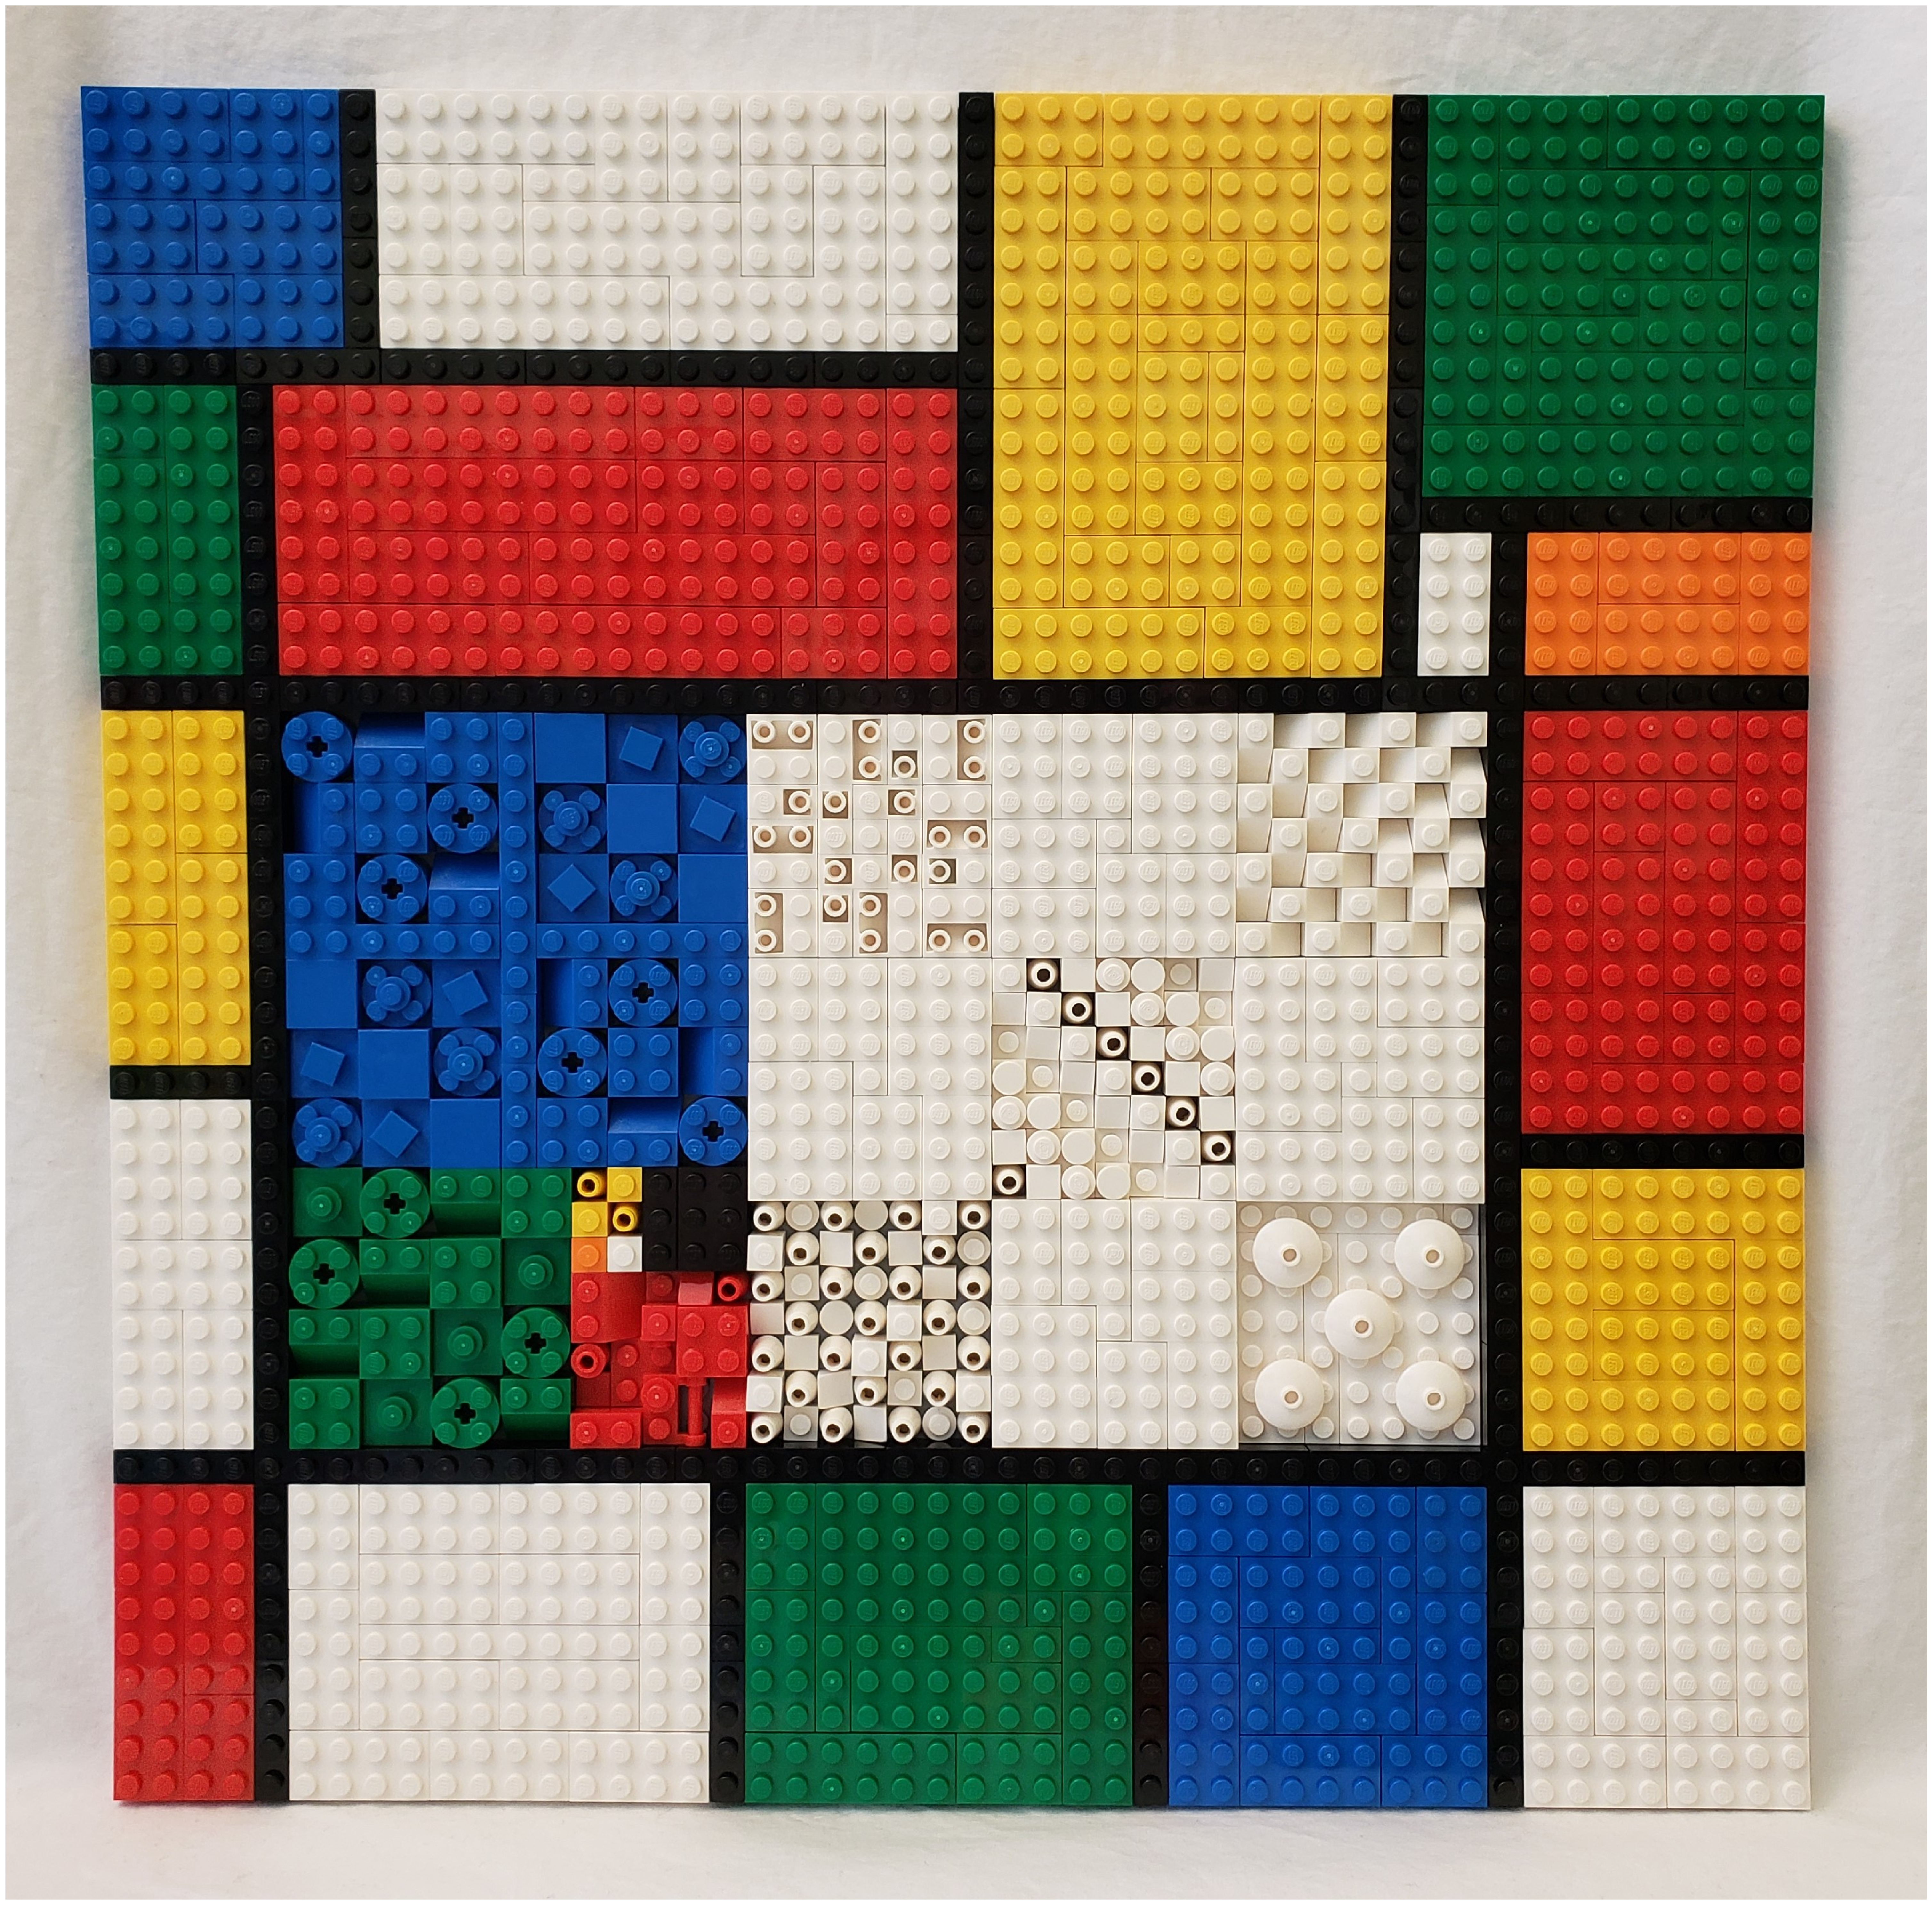
\includegraphics[width=.8\textwidth]{fig/FibonacciMondrian}
%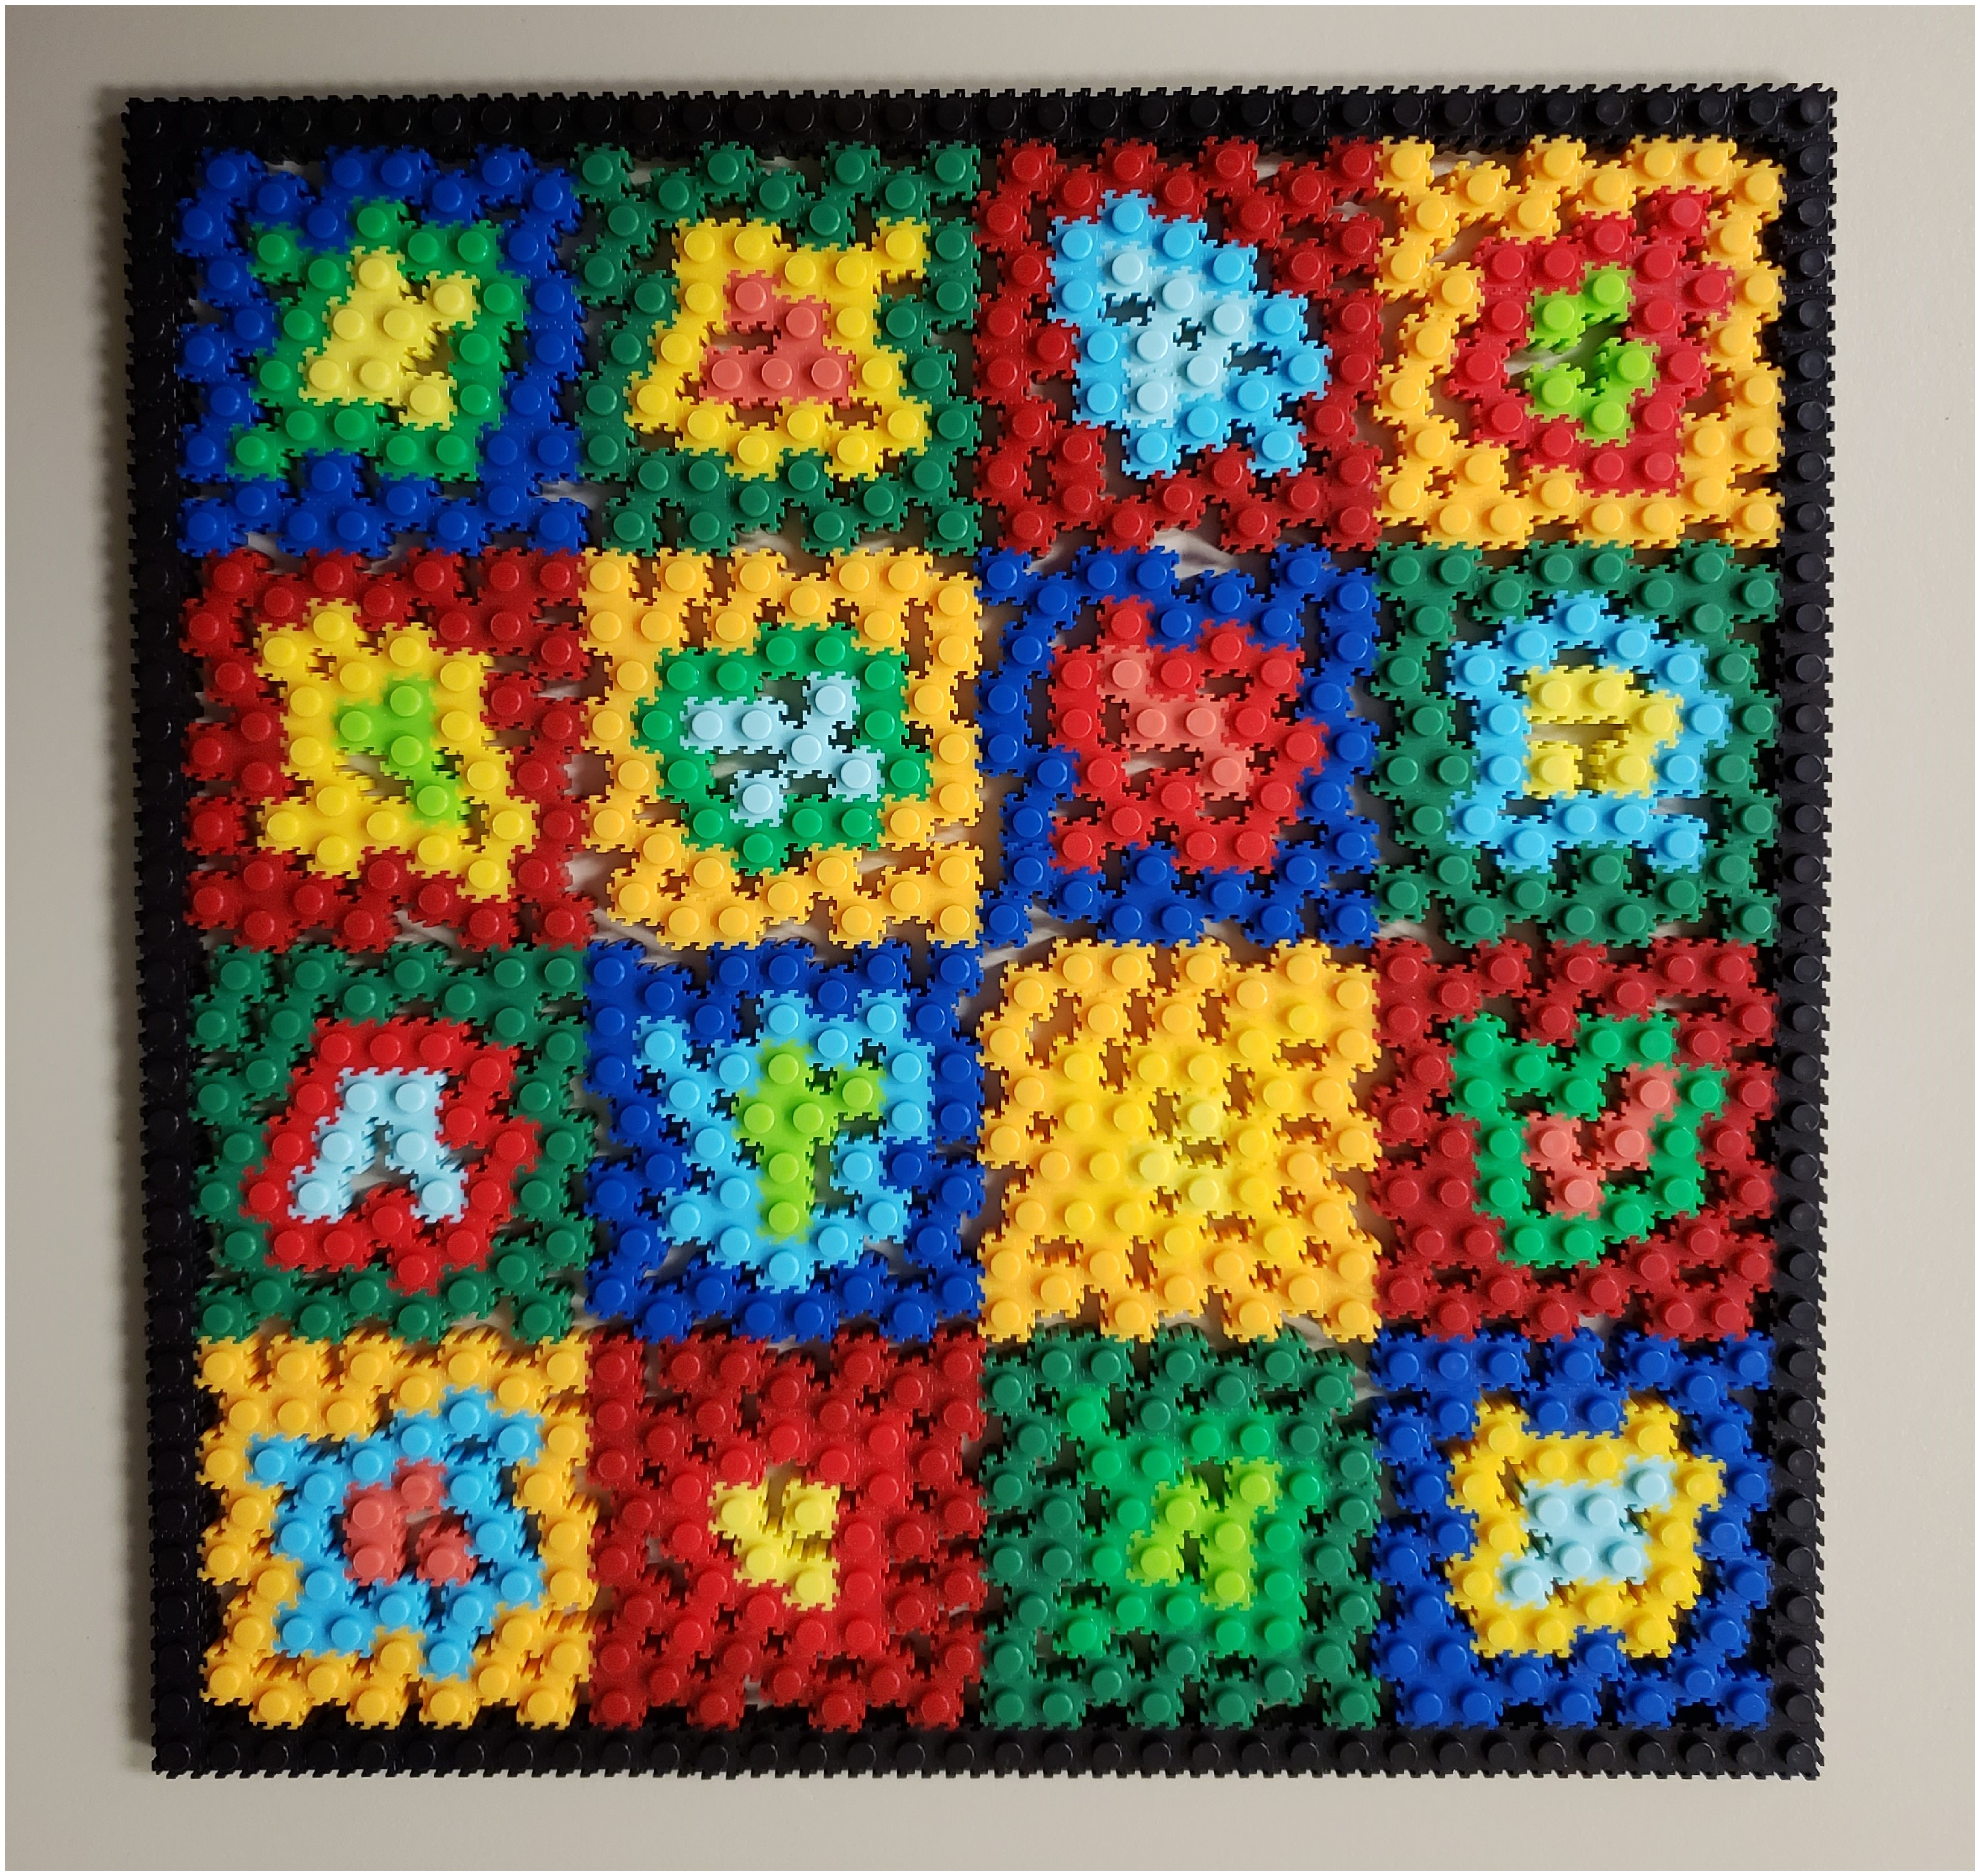
\includegraphics[width=.8\textwidth]{fig/2021Cover}
%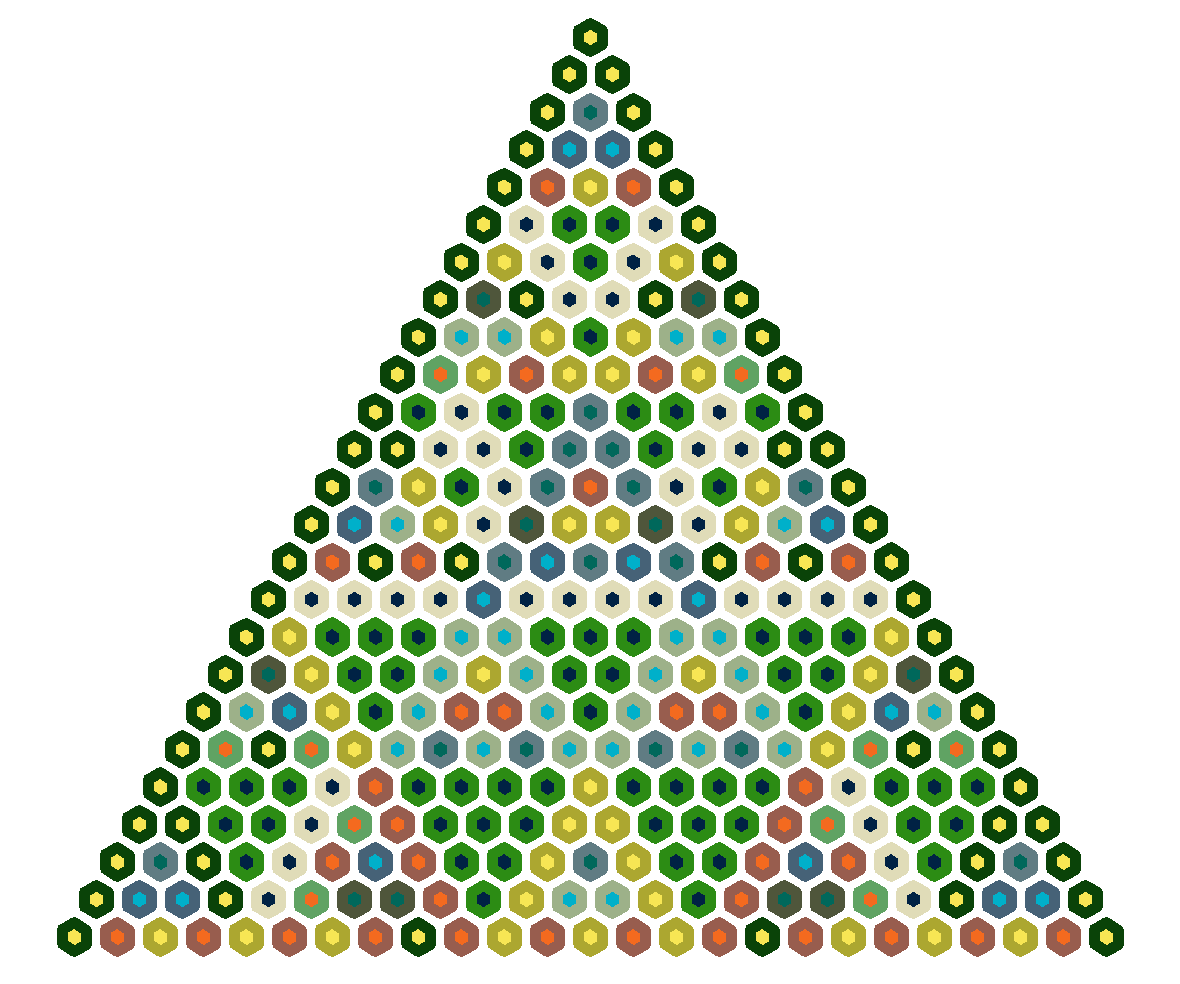
\includegraphics[width=\textwidth]{fig/PascalCover}
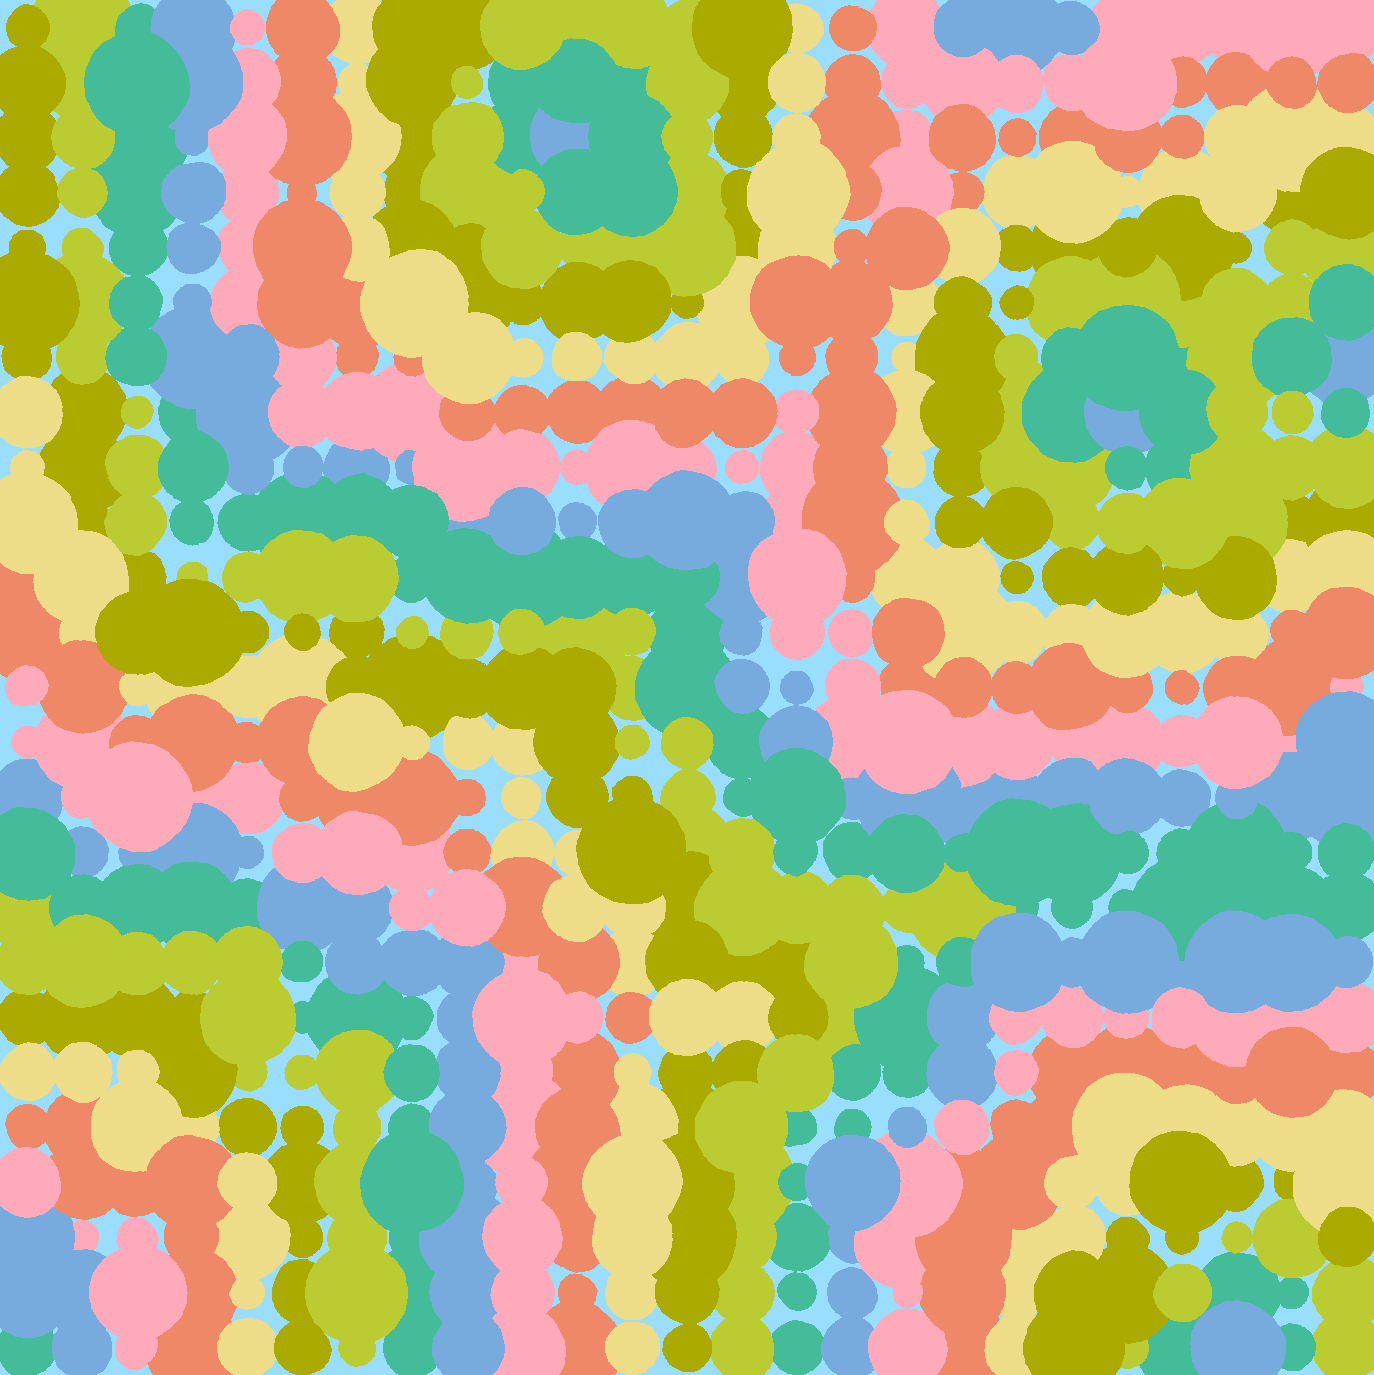
\includegraphics[width=.8\textwidth]{fig/SpotsCover}
}
\author{Charles A. Cusack\\
\href{mailto:cusack@hope.edu}{cusack@hope.edu}
%David A. Santos
}

\date{Version 3.5\\ \today}

\makeatletter
\newcommand{\twocoltoc}{%
  \section*{\contentsname
      \@mkboth{%
        }{}}%
  \begin{multicols}{2}\columnseprule 1pt \columnsep 25pt\multicoltolerance=900\small
    \@starttoc{toc}%
  \end{multicols}}
\makeatother

\usepackage{makeidx}
\makeindex
\usepackage[totoc]{idxlayout}


\setcounter{chapter}{-1}

%\input cap_c.tex
%%%%%%                  And voil� the document !!!
\begin{document}
% Front matter may follow here
\begin{frontmatter}
 \maketitle

\begin{quote}
    Copyright \copyright{}  2024  Charles A. Cusack.
    Permission is granted to copy, distribute and/or modify this document
    under the terms of the GNU Free Documentation License, Version 1.2
    or any later version published by the Free Software Foundation;
    with no Invariant Sections, no Front-Cover Texts, and no Back-Cover Texts.
    A copy of the license is included in the section entitled ``GNU
    Free Documentation License''.
\end{quote}
\begin{quote}
    Copyright \copyright{}  2007  David Anthony Santos.
    Permission is granted to copy, distribute and/or modify this document
    under the terms of the GNU Free Documentation License, Version 1.2
    or any later version published by the Free Software Foundation;
    with no Invariant Sections, no Front-Cover Texts, and no Back-Cover Texts.
    A copy of the license is included in the section entitled ``GNU
    Free Documentation License''.
\end{quote}


{\bf History}
%\markboth{}{} 
%\addcontentsline{toc}{chapter}{History}
%\markright{History}
\begin{itemize}
\item 2024:
Added sections on Matrices and Minimum Spanning Trees.
Increased coverage of modular arithmetic, including GCD and
Euclid's algorithm. 
Improved some of the coverage of algorithms topics.
Added matrix related problems to several chapters.
Various other minor changes throughout.
\item 2023: 
Reordered content, moved some of the proof content throughout so it can be used in a course
that does not want to be as proof focused.  Edited History to make it shorter.
\item 2021: 
More edits, added solutions to Reading Questions.
\item 2020:
Addition of Reading Comprehension Questions. 
Added material in Chapters 2, 4, 5, and especially 10. 
A few new Problems in several chapters. Minor edits throughout.
\item 2017, 2018, 2019:
Minor revisions/fixing of errors. A few additions/subtractions of material.
\item 2016:
Minor revisions.  Algorithm Analysis chapter had a few additions.
\item 2015:
Minor revisions.  Algorithm Analysis chapter had major revisions.
\item 2014:
A significant revision of the 2013 version, so a title change.
\item 2013: Original version titled {\em An Introduction to Discrete Mathematics and Algorithms}:
%%%\item
This document draws some content from each of the following. 
\begin{itemize}
\item Discrete Mathematics Notes, 2008, David A. Santos.
\item More Discrete Mathematics, 2007, David A. Santos.
\item Number Theory for Mathematical Contests, 2007, David A. Santos.
\item Linear Algebra Notes, 2008, David A. Santos.
\item Precalculus, An Honours Course, 2008, David Santos.
\end{itemize}
These documents used to be available from  
\href{http://www.opensourcemath.org/books/santos/}{http://www.opensourcemath.org/books/santos/},
but the site appears to no longer be available.
\end{itemize}

\vspace*{.25in}
\noindent
{\bf About the cover}

\noindent
Spots with almost circles of various sizes
using the Tol light color palette.
Created by Charles Cusack. 
For more of Dr. Cusack's digital art, go to 
\href{https://cusack.hope.edu/Art/}{https://cusack.hope.edu/Art/}

\newpage
{\normalsize
\twocoltoc{}
%\tableofcontents{}
}
\chapter*{Note to Instructors}
\addcontentsline{toc}{chapter}{Preface and Note to Instructors}

The latest version of this book is an attempt at making this textbook
more applicable in a wider range of courses. 
Although it was originally designed for use in a follow-up course 
to a data structures course for computer science majors,
the current version can also be used for a discrete mathematics
course with few to no prerequisites, and can be more or less focused
on proof writing according the the needs of a course.

The book was 
reorganized and has had content added to make it suitable for
a discrete mathematics course with no prerequisites for 
secondary mathematics education students in the state of Michigan
while continuing to serve the computer science students. 
I will be testing it in Spring 2025 for the first time with a mixed group
of secondary mathematics education, computer science, 
and potentially general education students.

Several changes were made in the past few versions to accomplish the
goals stated above.
The content was rearranged to allow a course 
to focus on proof writing or not. 
For instance, 
Sections \ref{section:setProofs}, 
\ref{section:functionProofs}, 
\ref{subsec:alProof}, 
and
\ref{subsec:limproof}
separate proofs involving
sets, functions, and computational complexity so they can be skipped if desired.
In fact, I currently teach a version of the course that is
not proof focused and we skip the entirety of Chapter~\ref{ch:proofs} 
on proofs along with those sections, yet we are still able to cover
induction proofs and the students seem to still pick up on that technique.

I also attempted to provide more details 
about topics I previously expected were review 
(e.g. programming fundamentals, sorting and searching algorithms, matrices),
and in a few places I note 
that examples or sections can be skipped based on 
the reader's background 
(e.g. Section~\ref{subsec:BDS} on basic data structures).
In addition, a section on minimum spanning trees 
was added so that non-computer science students would see 
at least one interesting example of a graph problem and
several algorithms to solve it.

Since the textbook has gone through some major changes in the past
few years, I definitely appreciate any feedback, positive or negative
(preferably constructive, though!), so that I can continue 
improving it. So if you see things that seem out of place, 
topics that you think should be there,
notice other problems, or have suggestions, please let me know.

In the past I have used this textbook for a discrete mathematics course
for computer science students with a data structures prerequisite and 
have covered the vast majority of the textbook.
As mentioned above, it will be used for a no-prerequisite discrete mathematics course for secondary
mathematics education students in Spring 2025. The current planned coverage is as follows
\begin{itemize}
\item 
Sections \ref{section:logic}-\ref{section:pred}
\item 
Sections \ref{section:sets}-\ref{section:functions} 
(skipping \ref{section:setProofs} and 
\ref{section:functionProofs})
\item Chapter \ref{ch:algs}
\item Chapter \ref{ch:seqsummat}
\item Chapter \ref{ch:AlgAn}
\item Chapter \ref{ch:recurrences} (skipping \ref{subsec:linear})
\item Chapter \ref{ch:count} (probably skipping \ref{sec:inclExcl})
\item Chapter \ref{ch:graphs}
\end{itemize}
%I am sad to say that I have not had sufficient time to map out 
%prerequisite sections or suggest which section may be useful in
%different sorts of courses. 
%I leave it in your capable hands to determine that for yourself.\\

Here is an anecdote on how I personally use the book that you might 
find helpful.
The \verb+TL;DR+ version: I have them answers all exercises
and reading questions before class
and their unanswered questions
are where each class period begins, and often lingers.
I rarely (never?) lecture through material when I use this textbook.
Students seem to like it and they are learning.

At the beginning of each semester, I have each student 
share a Google Doc with me called 
{\em Smith RQ}, where they replace {\em Smith} with their last name.
Every time I assign reading from the textbook,
I tell them to write answers to all of the exercises in the assigned sections
of the book (my students buy a printed copy of the book), 
and to put their answers to all of the reading questions into their 
Google Doc, placing the most recent answers at the top of the document
(to make it quicker for me to find).\footnote{
This could be done the old-fashioned way on pencil and paper, 
or by having them submit it via a CMS, but using 
a Google Doc means that the deadline is flexible and
they do not have to repeatedly turn their answers in since they 
just prepend them to the document they have already shared with me.}
I quickly go through their
documents to make sure they have filled out answers to the reading 
questions for the day, 
giving them 0-4 points depending on how they did.\footnote{Why
0-4? Since 4 is even, they can get half credit. And 5 categories seems
like a good number. The way I usually assign grades, 0-2 would also work
since very rarely do I give someone 1 or 3 points. But you do you.
}
For sake
of time, I only grade them based on attempt, not content.\footnote{I
think it is very important that students know when they are being graded
on effort instead of outcome since I never want them to get a sense that
they did something correct based on the fact that I did not mark it down.
I make it very clear to my students that it is their responsibility to grade
their own work and they need to ask questions if they are uncertain
about any of their answers.
} 
If they attempted to answer all of the questions 
(including answers such as ``I'm not sure how to do this one''),
they get 4 points. For half, they get 2. If they skip it, a big fat zero!
You get the idea.
When I have time, I do this before class so I can also take a brief look at 
some of the answers to get a sense of how the class is doing on the 
material.\footnote{
When my schedule allows me a free hour before class, I have the reading
questions due an hour before class. Other semester I have them due at 
midnight the night before or mid-morning to allow me time to look at 
them before class.}


At the beginning of class, I pick a random\footnote{
By ``random'' I really mean a page that is usually
in the second half of the reading and has multiple questions on it.
}
page from the reading 
that has exercises on it and ask all of them to show me their book. 
If they attempted to answer
all of the questions on the page (both displayed pages), they get 4 points.
If they tried some of them, they get 2 or 3. If they forgot to do it, they get 0.

I count these attempts as part of their grade so that they have motivation
to do it, but since the grades {\em should}
be fairly high on these, I do not want it to count for too much.
I call this category {\em Activities} or {\em Preparation}, and
it is often worth 15-20\% of their final grade. My exams and homework
are generally sufficiently difficult to compensate for the fact that many of 
the students will have really high scores in this category.

If one had access to a grader, a nice slight modification would be to
pick a handful of questions to grade for content, and the rest for completion.
That can work for both the exercises 
(they can put select answers in their Google Doc, for instance) 
and the reading questions. On the other hand, since 
answers to the exercises and reading questions are available in the book,
I am not sure that much is gained by grading these for content.

I spend the next part of class, and often the entire class, focusing
on answering questions from the exercises and reading questions that 
stumped them. 
I rarely lecture through material in this course. 
I expect that they will learn the mundane parts
(e.g. basic definitions) through reading, and we can
focus our time during class on the more complicated concepts and applying
the ideas. 

I have used this technique for over a decade and it seems to 
work well. In addition, most of my students appreciate the way the textbook 
is written and how I use it since it forces them to do the reading 
(that they otherwise would skip doing) and they 
get useful feedback along the way. On the other hand, they do mention 
that it is a lot of work---reading, answering exercises, and answering reading
questions takes a lot longer than just skimming, which is what many of them
would likely do otherwise. But in the end, they definitely seem to fall on 
the side of liking this approach.

\bigskip

\noindent
Charles A. Cusack

\noindent
June, 2024


%\chapter*{Preface}
%\addcontentsline{toc}{chapter}{Preface and Note to Instructors}
\newpage
\noindent{\LARGE \bf Preface}

\bigskip

This book is an attempt to present some of the most important discrete mathematics concepts
to computer science students in the context of algorithms.  I wrote it for use as a textbook
for half of a course on discrete mathematics and algorithms that we offer at Hope College.
Since it was written for use in this particular context,
it is important to note that the course (and therefore this book) 
has as a prerequisite what is typically referred to as CS2.
Thus, it is assumed that the reader has had one or more programming courses
(the example code in the book is very much like C++ or Java), 
has seen basic data structures (e.g. stacks, queues, linked lists, trees), 
has studied the standard sorting algorithms (e.g. selection sort, bubble sort,
insertion sort, Quicksort, and merge sort), 
and
has seen recursion (although that material is reviewed in the book). 
In addition, it is assumed that the reader has seen the binary representation of integers.
Finally, limits and derivatives are used in a few sections in the chapter on algorithm analysis
because I (and I think many students) find it much easier to prove bounds using limits
instead of the formal definitions, assuming they have had calculus. Because the majority of
our students have had calculus, I do not review those concepts. 
I have found that even the students who have not had calculus can tackle this material 
with a little extra help, especially given the fact that the derivatives and limits they need to 
compute are pretty straightforward. 
Alternatively, that section can be skipped 
(although it makes the next section on growth rates a bit more difficult to read in detail).

Some of the material is drawn from several open-source books by David Santos.
Other material is from handouts I have written and used over the years.  
I have extensively edited the material from both sources, 
both for clarity and to emphasize the connections
between the material and algorithms where possible.
I have also added a significant amount of new material.
The format of the material is also significantly different than it was in
the original sources.

I should mention that I never met David Santos, who apparently died in 2011. 
I stumbled upon his books in the summer  of 2013 when 
I was searching for a discrete mathematics book to use 
in a new course.  
When I discovered that I could adapt his material for my own use, I decided to do so.  
Since clearly he has no knowledge of this book, 
he bears no responsibility for any of the edited content.
Any errors or omissions are therefore mine.

I appreciate any feedback you have.  
Please send any typos, formatting errors, other errors, suggestions, etc., to  
\href{mailto:cusack@hope.edu}{cusack@hope.edu}.

I would like to thank the following people for submitting feedback/errata (listed in no particular order):
Dan Zingaro, 
Mike Jipping, 
Steve Ratering, 
Victoria Gonda, 
Nathan Vance, 
Cole Watson, 
Kalli Crandell, 
John Dood, 
James Cerone,
Coty Franklin, 
Kyle Magnuson, 
Karl-Dieter Crisman,
Katie Brudos, 
Jonathan Senning, 
Matthew DeJongh, 
Julian Payne, 
Josiah Brouwer,
Cole Bruns,
and probably several others I forgot to mention (sorry!).
I would like to especially thank Lydia Won for helping 
write/compile solutions for the reading comprehension questions.

\bigskip
\noindent
Charles A. Cusack

\noindent
May, 2019


\chapter*{Note to Students}
\addcontentsline{toc}{chapter}{Note to Students}

As the title of the book indicates, this is not a book that is just to be read.  It was written
so that the reader interacts with the material.  If you attempt to just read what is 
written and take no part in the exercises that are embedded throughout, you will likely
get very little out of it.  Learning needs to be active, not passive.  The more active you are
as you `read' the book, the more you will get out of it.  That will translate to better learning.
And it will also translate to a higher grade.  So whether you are motivated by learning (which is
my hope) or merely by getting a certain grade, your path will be the same--use this book as 
described below.

The content is presented in the following manner.  
First, concepts and definitions are given--generally one at a time.  
Then one or more examples that illustrate the concept/definition will be given.  
After that you will find one or more exercises of various kinds.  This is where this book
differs from most.  Instead of piling on more examples that you merely read and {\em think} you understand,
you will be asked to solve some for yourself so that you can be more confident that you really {\em do}
understand. 

Some of the exercises are just called {\em Exercises}.  
They are very similar to the examples, except that you have to provide the solution.  
There are also {\em Fill in the details} which provide part of the solution, but ask you to provide
some of the details.  The point of these is to help you think about some of the finer details that
you might otherwise miss.  There are also {\em Questions} of various kinds that get you thinking about
the concepts. Finally, there are {\em Evaluate} exercises.  These ask you to look at solutions written
by others and determine whether or not they are correct.  More precisely, your goal is to try to find
as many errors in the solutions as you can.  Usually there will be one or more errors in each solution,
but occasionally a correct solution will be given, so pay careful attention to every detail.  The point 
of these exercises is to help you see mistakes before you make them.  Many of these exercises are based
on solutions from previous students, so they often represent the common mistakes students make.
Hopefully if you see someone else make these mistakes, you will be less likely to make them yourself. 

The point of the exercises is to get you thinking about and interacting with the material.  
As you encounter these, you should write your solution in the space provided.  After you have written
your solution, you should check your answer with the solution provided in the back of the book.  
You will get the most out of them if you first do your
best to give a complete solution on your own, and then {\em always} check your solution with the one provided
to make sure you did it correctly.  If yours is significantly different, make sure you determine whether or
not the differences are just a matter of choice or if there is something wrong with your solution.

If you get stuck on an exercise, you should re-read the previous material 
(definitions, examples, etc.) and see if that helps.  Then give it a little more thought.  
For {\em Fill in the details} questions, sometimes reading what is past a blank will help you
figure out what to put there.
If you get {\em really} stuck on an exercise, look up the solution and make sure you fully understand it.  
But don't jump to the solution too quickly or too often without giving an honest attempt at solving the exercise
yourself.  When you do end up looking up a solution, you should always try to rewrite it in the
space provided {\em in your own words}.  
You should not just copy it word for word. You won't learn as 
much if you do that.  Instead, do your best to fully understand the solution.  Then, without looking
at the solution, try to re-solve the problem and write your solution in the space provided.  
Then check the solution again to make sure you got it right.

It is highly recommended that you act as your own grader when you check your solutions.
If your solution is correct, put a big check mark in the margin.  
If there are just a few errors, 
use a different colored writing utensil to mark and fix your errors.
If your solution is way off, cross it out (just put a big `X' through it) 
and write out your second attempt, using a separate sheet of paper if necessary. 
If you couldn't get very far without reading the solution, you should somehow indicate that. 
So that you can track your errors, I highly recommend crossing out incorrect solutions
(or portions of solutions) instead of erasing them.  
Doing this will also allow you to look back and determine how well you did as you were working
through each chapter.  
It may also help you determine how to spend your time as you study for exams. 

This whole process will help you become better at evaluating your own work. 
This is important because you should be confident in your answers, but only when they
are correct.  Grading yourself will help you gain confidence when you are correct and
help you quickly realize when you are not correct so that you do not
become confident about the wrong things.
Another reason that grading your solutions is important is so that when you go back
to re-read any portion of the book, you will know whether or not what you wrote
was correct.

It is important that you read the solutions to the exercises after you attempt them, even if you
think your solution is correct.  
The solutions often provide further insight into the material and should be regarded 
as part of any reading assignment given.

Make sure you read carefully.  When you come upon an {\em Evaluate} exercise, do not
mistake it for an example.  Doing so might lead you down the wrong path.  Never consider
the content of an {\em Evaluate} exercise to be correct unless you have verified with the 
solution that it is really correct.  To be safe, when re-reading, always assume that the
{\em Evaluate} exercises are incorrect, and never use them as a model for your own problem 
solving.  To help you, we have tried to differentiate these from other example and exercise
types by using a different font.

There is an expectation that you are able to solve every exercise on your own.
(Note that I am talking about the exercises embedded into the chapters, 
not the homework problems at the end of each chapter.)
If there are exercises that you are unable to complete, you need to get them cleared up
immediately.  This might mean asking about them in class, going to see the professor or a
teaching assistant, and/or going to a help center/tutor.  Whatever it takes, make sure you 
have a clear understanding of how to solve all of them.  

Every chapter ends with two sections called {\em Reading Comprehension Questions}
and {\em Problems}. The {\em Problems} sections are exactly what they sound like--a list of problems
suitable for working on in class or given as homework assignments.

All of the {\em Reading Comprehension Questions} should be attempted after
you have finished reading each section (including completing all of the exercises). 
They are sort of the final check of your comprehension of the material before you move on to solving 
homework problems.
Although some of these questions are similar to the exercises in the sections,
others are more conceptual in nature. The majority of them are not meant to be difficult, but rather to
test whether you really understand the material from the section as whole. These can be used as a starting point
for class discussion, so be sure to ask about those that you have trouble completing and/or are unsure about.

Space is not given in the book for solutions to the {\em Reading Comprehension Questions}, 
so write your answers on paper or use a Google Doc or other typesetting software to record your solutions.
(In my classes I have students share a Google Doc with me in which they place their answers to these questions,
adding the most recent answers at the top of the document to make it easier to find their recent answers.
When questions can't easily be done in a Google Doc, they write their solution on paper, scan or take a picture of it, 
and include the picture in their Google Doc.)

Solutions to the {\em Reading Comprehension Questions} are available in the back of the book.
As with the exercises throughout the book, it is highly recommended that you check your answers and grade 
your own work, crossing out your solution when you were incorrect (instead of erasing/deleting it)
and replacing it with the correct solution.



\end{frontmatter}

\clearpage
% This makes it print another page number at the bottom.
% I never noticed that.  It doesn't seem to do much else that I can see.
% I think it also prints lines at the bottom and top of the page.
%CAC, 9/2/14
%\pagestyle{fancy}

\renewcommand{\headrulewidth}{1pt}
\renewcommand{\footrulewidth}{1pt}
\lhead[\rm\thepage]{\nouppercase{\textcolor{blue}{\it\rightmark}}}
\rhead[\nouppercase{\textcolor{blue}{\it\leftmark}}]{\rm \thepage}
\renewcommand{\chaptermark}[0]{\markboth{\chaptername\ \thechapter}}
\renewcommand{\sectionmark}{\markright}
\pagenumbering{arabic} 
\setcounter{page}{1} 

\includechapter{motivation}
\includechapter{logic}
\includechapter{proofs}
\includechapter{setsFunctionsRelations}
\includechapter{algorithms}
\includechapter{sequencesAndSummations}
\includechapter{algorithmAnalysis}
\includechapter{recurrencesRecursionInduction}
\includechapter{counting}
\includechapter{graphs}

\chapter*{Reading Question Solutions}
\phantomsection  % so hyperref creates bookmarks
\addcontentsline{toc}{chapter}{Reading Question Solutions}
\includeRQsolutions{logic}
\includeRQsolutions{proofs}
\includeRQsolutions{setsFunctionsRelations}
\includeRQsolutions{algorithms}
\includeRQsolutions{sequencesAndSummations}
\includeRQsolutions{algorithmAnalysis}
\includeRQsolutions{recurrencesRecursionInduction}
\includeRQsolutions{counting}
\includeRQsolutions{graphs}


\chapter*{Exercise Solutions}
\phantomsection  % so hyperref creates bookmarks
\addcontentsline{toc}{chapter}{Exercise Solutions}
\includesolutions{logic}
\includesolutions{proofs}
\includesolutions{setsFunctionsRelations}
\includesolutions{algorithms}
\includesolutions{sequencesAndSummations}
\includesolutions{algorithmAnalysis}
\includesolutions{recurrencesRecursionInduction}
\includesolutions{counting}
\includesolutions{graphs}

%%%%%
% The GNU Documentation license.
\clearpage
{\tiny
\input{misc/fdl-1.2.tex}
}

\printindex

\end{document}
